
\begin{figure*}[t]
\centering
\tikzset{every picture/.style={line width=0.75pt}} %set default line width to 0.75pt

\scalebox{0.7}{










\tikzset{every picture/.style={line width=0.9pt}} %set default line width to 0.75pt

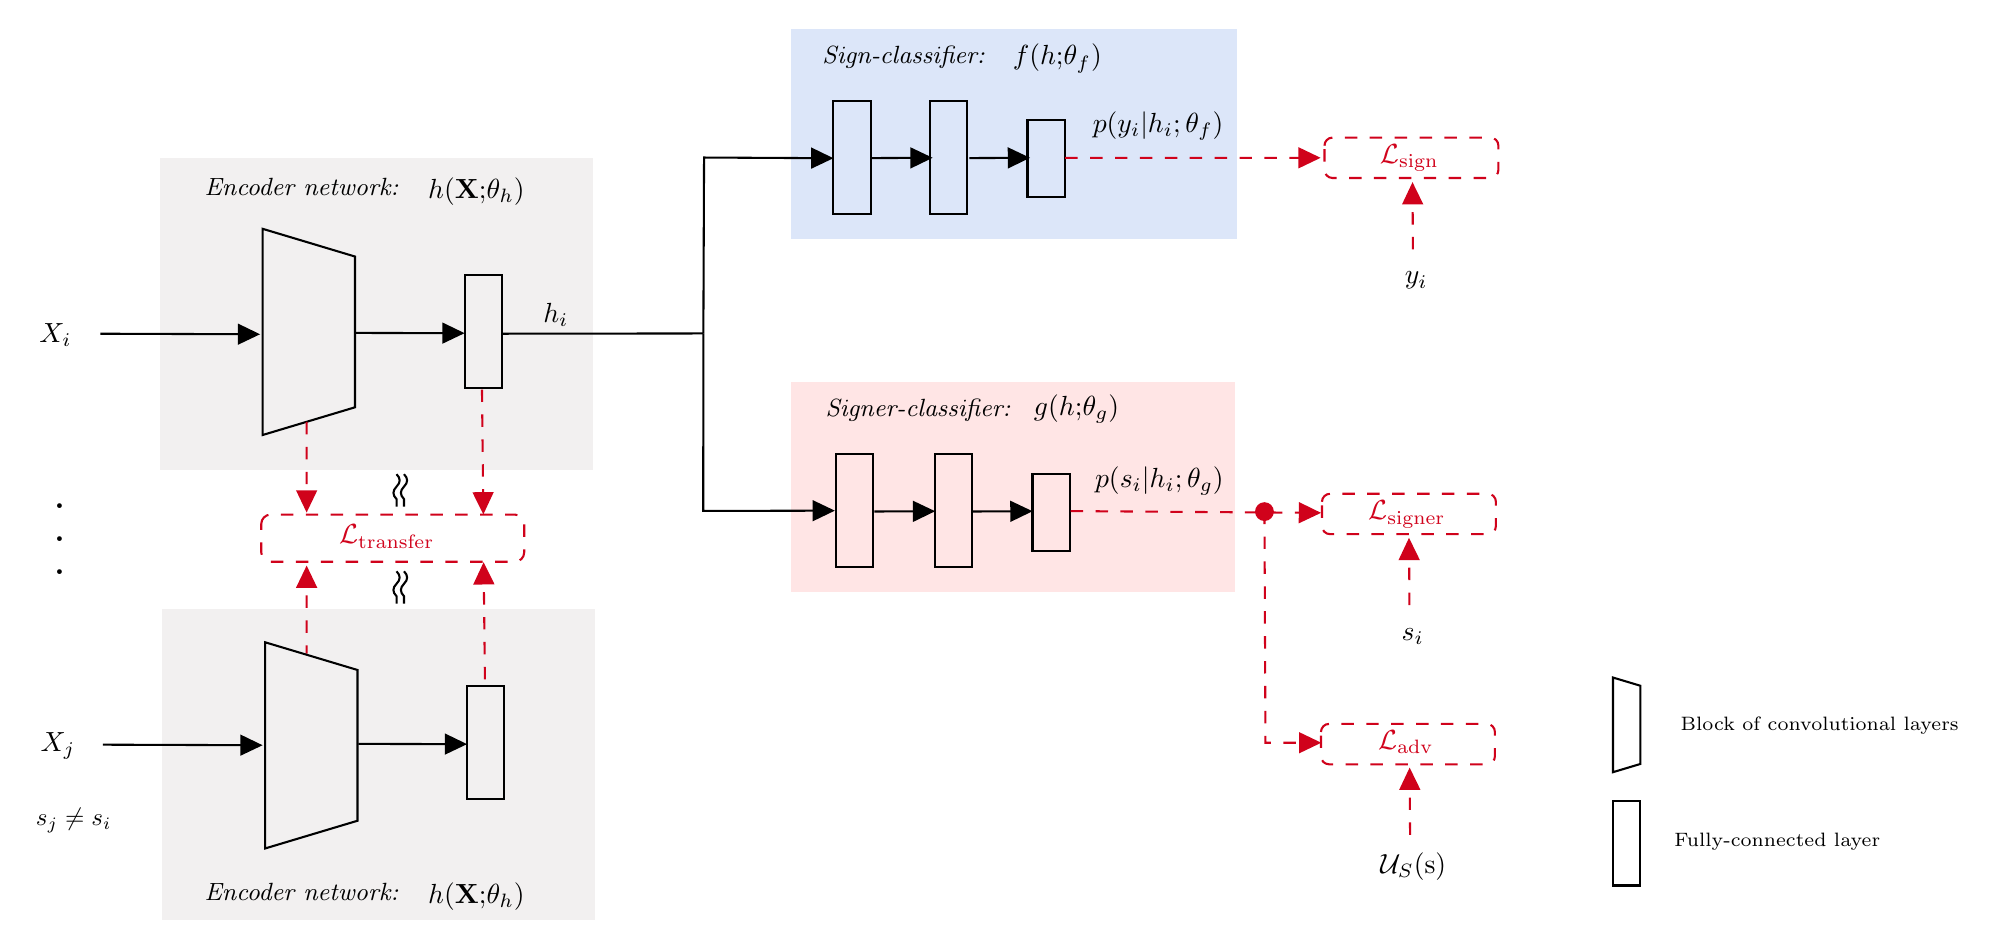
\begin{tikzpicture}[x=0.9pt,y=0.9pt,yscale=-1,xscale=1]
%uncomment if require: \path (0,637); %set diagram left start at 0, and has height of 637

%Shape: Rectangle [id:dp7817430644997849]
\draw  [draw opacity=0][fill={rgb, 255:red, 226; green, 223; blue, 223 }  ,fill opacity=0.46 ][dash pattern={on 4.5pt off 4.5pt}] (89.57,241.83) -- (263.45,241.83) -- (263.45,367) -- (89.57,367) -- cycle ;
%Shape: Rectangle [id:dp43448545781433445]
\draw  [draw opacity=0][fill={rgb, 255:red, 124; green, 163; blue, 233 }  ,fill opacity=0.27 ][dash pattern={on 4.5pt off 4.5pt}] (342,9) -- (521,9) -- (521,93.23) -- (342,93.23) -- cycle ;
%Shape: Rectangle [id:dp47448290384115754]
\draw  [draw opacity=0][fill={rgb, 255:red, 226; green, 223; blue, 223 }  ,fill opacity=0.46 ][dash pattern={on 4.5pt off 4.5pt}] (88.57,60.83) -- (262.45,60.83) -- (262.45,186) -- (88.57,186) -- cycle ;
%Shape: Trapezoid [id:dp7544890433922595]
\draw   (129.83,89.34) -- (166.92,100.47) -- (166.92,161) -- (129.83,172.13) -- cycle ;
%Shape: Rectangle [id:dp07852532899632947]
\draw   (225.83,108) -- (225.83,153.36) -- (210.91,153.36) -- (210.91,108) -- cycle ;
%Straight Lines [id:da6483299081027241]
\draw    (167.27,131.14) -- (208.91,131.24) ;
\draw [shift={(210.91,131.24)}, rotate = 180.14] [fill={rgb, 255:red, 0; green, 0; blue, 0 }  ][line width=0.75]  [draw opacity=0] (8.93,-4.29) -- (0,0) -- (8.93,4.29) -- cycle    ;

%Straight Lines [id:da3383332186453154]
\draw    (64.69,131.46) -- (126.8,131.67) ;
\draw [shift={(128.8,131.68)}, rotate = 180.19] [fill={rgb, 255:red, 0; green, 0; blue, 0 }  ][line width=0.75]  [draw opacity=0] (8.93,-4.29) -- (0,0) -- (8.93,4.29) -- cycle    ;

%Straight Lines [id:da8976159443553993]
\draw    (225.86,131.46) -- (306.79,131.35) ;


%Shape: Rectangle [id:dp39844785350453726]
\draw   (373.93,38.03) -- (373.93,83.38) -- (359.01,83.38) -- (359.01,38.03) -- cycle ;
%Shape: Rectangle [id:dp5960148926786581]
\draw   (412.75,38.03) -- (412.75,83.38) -- (397.84,83.38) -- (397.84,38.03) -- cycle ;
%Shape: Rectangle [id:dp2968748699957451]
\draw   (451.86,45.72) -- (451.86,76.69) -- (436.94,76.69) -- (436.94,45.72) -- cycle ;
%Straight Lines [id:da38135442637321804]
\draw    (374.47,60.94) -- (396.84,60.84) ;
\draw [shift={(398.84,60.83)}, rotate = 539.75] [fill={rgb, 255:red, 0; green, 0; blue, 0 }  ][line width=0.75]  [draw opacity=0] (8.93,-4.29) -- (0,0) -- (8.93,4.29) -- cycle    ;

%Straight Lines [id:da5103446228646831]
\draw    (413.57,60.94) -- (435.94,60.84) ;
\draw [shift={(437.94,60.83)}, rotate = 539.75] [fill={rgb, 255:red, 0; green, 0; blue, 0 }  ][line width=0.75]  [draw opacity=0] (8.93,-4.29) -- (0,0) -- (8.93,4.29) -- cycle    ;

%Shape: Rectangle [id:dp21504155648063916]
\draw  [draw opacity=0][fill={rgb, 255:red, 255; green, 199; blue, 199 }  ,fill opacity=0.46 ][dash pattern={on 4.5pt off 4.5pt}] (342.06,150.9) -- (520.25,150.9) -- (520.25,235.13) -- (342.06,235.13) -- cycle ;
%Shape: Rectangle [id:dp5629086137047858]
\draw   (374.93,179.92) -- (374.93,225.28) -- (360.01,225.28) -- (360.01,179.92) -- cycle ;
%Shape: Rectangle [id:dp11383387176162141]
\draw   (414.75,179.92) -- (414.75,225.28) -- (399.84,225.28) -- (399.84,179.92) -- cycle ;
%Shape: Rectangle [id:dp8834314863600405]
\draw   (453.86,187.61) -- (453.86,218.59) -- (438.94,218.59) -- (438.94,187.61) -- cycle ;
%Straight Lines [id:da7960584409422926]
\draw    (375.47,202.84) -- (397.84,202.74) ;
\draw [shift={(399.84,202.73)}, rotate = 539.75] [fill={rgb, 255:red, 0; green, 0; blue, 0 }  ][line width=0.75]  [draw opacity=0] (8.93,-4.29) -- (0,0) -- (8.93,4.29) -- cycle    ;

%Straight Lines [id:da26603179330471005]
\draw    (414.57,202.84) -- (436.94,202.74) ;
\draw [shift={(438.94,202.73)}, rotate = 539.75] [fill={rgb, 255:red, 0; green, 0; blue, 0 }  ][line width=0.75]  [draw opacity=0] (8.93,-4.29) -- (0,0) -- (8.93,4.29) -- cycle    ;

%Straight Lines [id:da645470302869213]
\draw    (306.79,131.35) -- (307.07,60.72) -- (357,60.99) ;
\draw [shift={(359,61)}, rotate = 180.31] [fill={rgb, 255:red, 0; green, 0; blue, 0 }  ][line width=0.75]  [draw opacity=0] (8.93,-4.29) -- (0,0) -- (8.93,4.29) -- cycle    ;

%Straight Lines [id:da6326177139350364]
\draw    (306.79,131.35) -- (306.74,202.61) -- (357.56,202.5) ;
\draw [shift={(359.56,202.5)}, rotate = 539.88] [fill={rgb, 255:red, 0; green, 0; blue, 0 }  ][line width=0.75]  [draw opacity=0] (8.93,-4.29) -- (0,0) -- (8.93,4.29) -- cycle    ;

%Straight Lines [id:da43094599217232044]
\draw [color={rgb, 255:red, 208; green, 2; blue, 27 }  ,draw opacity=1 ] [dash pattern={on 4.5pt off 4.5pt}]  (452.06,60.88) -- (552.61,60.84) ;
\draw [shift={(554.61,60.83)}, rotate = 539.98] [fill={rgb, 255:red, 208; green, 2; blue, 27 }  ,fill opacity=1 ][line width=0.75]  [draw opacity=0] (8.93,-4.29) -- (0,0) -- (8.93,4.29) -- cycle    ;

%Rounded Rect [id:dp20102262667247417]
\draw  [color={rgb, 255:red, 208; green, 2; blue, 27 }  ,draw opacity=1 ][dash pattern={on 4.5pt off 4.5pt}] (555.16,198.96) .. controls (555.16,197.16) and (556.62,195.71) .. (558.41,195.71) -- (621.75,195.71) .. controls (623.55,195.71) and (625,197.16) .. (625,198.96) -- (625,208.69) .. controls (625,210.48) and (623.55,211.94) .. (621.75,211.94) -- (558.41,211.94) .. controls (556.62,211.94) and (555.16,210.48) .. (555.16,208.69) -- cycle ;
%Straight Lines [id:da7107772326187543]
\draw [color={rgb, 255:red, 208; green, 2; blue, 27 }  ,draw opacity=1 ] [dash pattern={on 4.5pt off 4.5pt}]  (454.25,202.67) -- (552.78,203.37) ;
\draw [shift={(554.78,203.38)}, rotate = 180.41] [fill={rgb, 255:red, 208; green, 2; blue, 27 }  ,fill opacity=1 ][line width=0.75]  [draw opacity=0] (8.93,-4.29) -- (0,0) -- (8.93,4.29) -- cycle    ;

%Straight Lines [id:da7856916848123423]
\draw [color={rgb, 255:red, 208; green, 2; blue, 27 }  ,draw opacity=1 ] [dash pattern={on 4.5pt off 4.5pt}]  (147.5,166.88) -- (147.51,201.24) ;
\draw [shift={(147.51,203.24)}, rotate = 269.99] [fill={rgb, 255:red, 208; green, 2; blue, 27 }  ,fill opacity=1 ][line width=0.75]  [draw opacity=0] (8.93,-4.29) -- (0,0) -- (8.93,4.29) -- cycle    ;

%Straight Lines [id:da899109719860808]
\draw [color={rgb, 255:red, 208; green, 2; blue, 27 }  ,draw opacity=1 ] [dash pattern={on 4.5pt off 4.5pt}]  (217.9,153.87) -- (218.43,202) ;
\draw [shift={(218.45,204)}, rotate = 269.36] [fill={rgb, 255:red, 208; green, 2; blue, 27 }  ,fill opacity=1 ][line width=0.75]  [draw opacity=0] (8.93,-4.29) -- (0,0) -- (8.93,4.29) -- cycle    ;

%Straight Lines [id:da36002582240035363]
\draw [color={rgb, 255:red, 0; green, 0; blue, 0 }  ,draw opacity=1 ][line width=0.75]    (186.6,226.85) .. controls (188.27,228.52) and (188.27,230.18) .. (186.6,231.85) .. controls (184.93,233.52) and (184.93,235.18) .. (186.6,236.85) -- (186.6,239.85) -- (186.6,239.85)(183.6,226.85) .. controls (185.27,228.52) and (185.27,230.18) .. (183.6,231.85) .. controls (181.93,233.52) and (181.93,235.18) .. (183.6,236.85) -- (183.6,239.85) -- (183.6,239.85) ;


%Rounded Rect [id:dp28118263286951617]
\draw  [color={rgb, 255:red, 208; green, 2; blue, 27 }  ,draw opacity=1 ][dash pattern={on 4.5pt off 4.5pt}] (556.16,55.96) .. controls (556.16,54.16) and (557.62,52.71) .. (559.41,52.71) -- (622.75,52.71) .. controls (624.55,52.71) and (626,54.16) .. (626,55.96) -- (626,65.69) .. controls (626,67.48) and (624.55,68.94) .. (622.75,68.94) -- (559.41,68.94) .. controls (557.62,68.94) and (556.16,67.48) .. (556.16,65.69) -- cycle ;
%Straight Lines [id:da5356763271282314]
\draw [color={rgb, 255:red, 208; green, 2; blue, 27 }  ,draw opacity=1 ] [dash pattern={on 4.5pt off 4.5pt}]  (591.52,72.62) -- (591.71,101.6) ;

\draw [shift={(591.51,70.62)}, rotate = 89.63] [fill={rgb, 255:red, 208; green, 2; blue, 27 }  ,fill opacity=1 ][line width=0.75]  [draw opacity=0] (8.93,-4.29) -- (0,0) -- (8.93,4.29) -- cycle    ;
%Straight Lines [id:da9155638065763507]
\draw [color={rgb, 255:red, 208; green, 2; blue, 27 }  ,draw opacity=1 ] [dash pattern={on 4.5pt off 4.5pt}]  (590.12,215.42) -- (590.31,244.4) ;

\draw [shift={(590.11,213.42)}, rotate = 89.63] [fill={rgb, 255:red, 208; green, 2; blue, 27 }  ,fill opacity=1 ][line width=0.75]  [draw opacity=0] (8.93,-4.29) -- (0,0) -- (8.93,4.29) -- cycle    ;
%Straight Lines [id:da7191094178180941]
\draw [color={rgb, 255:red, 0; green, 0; blue, 0 }  ,draw opacity=1 ][line width=0.75]    (186.6,187.85) .. controls (188.27,189.52) and (188.27,191.18) .. (186.6,192.85) .. controls (184.93,194.52) and (184.93,196.18) .. (186.6,197.85) -- (186.6,200.85) -- (186.6,200.85)(183.6,187.85) .. controls (185.27,189.52) and (185.27,191.18) .. (183.6,192.85) .. controls (181.93,194.52) and (181.93,196.18) .. (183.6,197.85) -- (183.6,200.85) -- (183.6,200.85) ;


%Straight Lines [id:da9896530377071313]
\draw [color={rgb, 255:red, 208; green, 2; blue, 27 }  ,draw opacity=1 ] [dash pattern={on 4.5pt off 4.5pt}]  (147.51,226.56) -- (147.5,259.88) ;

\draw [shift={(147.51,224.56)}, rotate = 90.02] [fill={rgb, 255:red, 208; green, 2; blue, 27 }  ,fill opacity=1 ][line width=0.75]  [draw opacity=0] (8.93,-4.29) -- (0,0) -- (8.93,4.29) -- cycle    ;
%Shape: Trapezoid [id:dp6458709768563871]
\draw   (672,269.5) -- (683,272.8) -- (683,304.2) -- (672,307.5) -- cycle ;
%Shape: Rectangle [id:dp1901046474760686]
\draw   (226.83,273) -- (226.83,318.36) -- (211.91,318.36) -- (211.91,273) -- cycle ;
%Straight Lines [id:da8673211689855849]
\draw    (168.27,296.14) -- (209.91,296.24) ;
\draw [shift={(211.91,296.24)}, rotate = 180.14] [fill={rgb, 255:red, 0; green, 0; blue, 0 }  ][line width=0.75]  [draw opacity=0] (8.93,-4.29) -- (0,0) -- (8.93,4.29) -- cycle    ;

%Straight Lines [id:da3618642920648949]
\draw    (65.69,296.46) -- (127.8,296.67) ;
\draw [shift={(129.8,296.68)}, rotate = 180.19] [fill={rgb, 255:red, 0; green, 0; blue, 0 }  ][line width=0.75]  [draw opacity=0] (8.93,-4.29) -- (0,0) -- (8.93,4.29) -- cycle    ;

%Rounded Rect [id:dp5531536926433998]
\draw  [color={rgb, 255:red, 208; green, 2; blue, 27 }  ,draw opacity=1 ][dash pattern={on 4.5pt off 4.5pt}] (129.28,207.86) .. controls (129.28,205.77) and (130.98,204.07) .. (133.07,204.07) -- (231.08,204.07) .. controls (233.17,204.07) and (234.86,205.77) .. (234.86,207.86) -- (234.86,219.21) .. controls (234.86,221.31) and (233.17,223) .. (231.08,223) -- (133.07,223) .. controls (130.98,223) and (129.28,221.31) .. (129.28,219.21) -- cycle ;
%Straight Lines [id:da5399866438305847]
\draw [color={rgb, 255:red, 208; green, 2; blue, 27 }  ,draw opacity=1 ] [dash pattern={on 4.5pt off 4.5pt}]  (218.58,225.21) -- (219.12,273.33) ;

\draw [shift={(218.56,223.21)}, rotate = 89.36] [fill={rgb, 255:red, 208; green, 2; blue, 27 }  ,fill opacity=1 ][line width=0.75]  [draw opacity=0] (8.93,-4.29) -- (0,0) -- (8.93,4.29) -- cycle    ;
%Straight Lines [id:da6744189660599909]
\draw [color={rgb, 255:red, 208; green, 2; blue, 27 }  ,draw opacity=1 ] [dash pattern={on 4.5pt off 4.5pt}]  (532.07,202.88) -- (532.47,295.68) -- (552.87,295.68) ;
\draw [shift={(554.87,295.68)}, rotate = 180] [fill={rgb, 255:red, 208; green, 2; blue, 27 }  ,fill opacity=1 ][line width=0.75]  [draw opacity=0] (8.93,-4.29) -- (0,0) -- (8.93,4.29) -- cycle    ;
\draw [shift={(532.07,202.88)}, rotate = 89.75] [color={rgb, 255:red, 208; green, 2; blue, 27 }  ,draw opacity=1 ][fill={rgb, 255:red, 208; green, 2; blue, 27 }  ,fill opacity=1 ][line width=0.75]      (0, 0) circle [x radius= 3.35, y radius= 3.35]   ;
%Rounded Rect [id:dp27586876312894315]
\draw  [color={rgb, 255:red, 208; green, 2; blue, 27 }  ,draw opacity=1 ][dash pattern={on 4.5pt off 4.5pt}] (554.76,291.36) .. controls (554.76,289.56) and (556.22,288.11) .. (558.01,288.11) -- (621.35,288.11) .. controls (623.15,288.11) and (624.6,289.56) .. (624.6,291.36) -- (624.6,301.09) .. controls (624.6,302.88) and (623.15,304.34) .. (621.35,304.34) -- (558.01,304.34) .. controls (556.22,304.34) and (554.76,302.88) .. (554.76,301.09) -- cycle ;
%Straight Lines [id:da05722319267703546]
\draw [color={rgb, 255:red, 208; green, 2; blue, 27 }  ,draw opacity=1 ] [dash pattern={on 4.5pt off 4.5pt}]  (590.37,307.67) -- (590.56,336.65) ;

\draw [shift={(590.36,305.67)}, rotate = 89.63] [fill={rgb, 255:red, 208; green, 2; blue, 27 }  ,fill opacity=1 ][line width=0.75]  [draw opacity=0] (8.93,-4.29) -- (0,0) -- (8.93,4.29) -- cycle    ;
%Shape: Trapezoid [id:dp41106407745048745]
\draw   (130.83,255.34) -- (167.92,266.47) -- (167.92,327) -- (130.83,338.13) -- cycle ;
%Shape: Rectangle [id:dp5258454923666749]
\draw   (683,319) -- (683,353) -- (671.91,353) -- (671.91,319) -- cycle ;

% Text Node
\draw (46.68,132.11) node   {$\boldsymbol{X}_{i}$};
% Text Node
\draw (48.35,213.89) node  [align=left] {\textbf{{\large .}}\\\textbf{{\large .}}\\\textbf{{\large .}}};
% Text Node
\draw (145.74,72.5) node  [align=left] {{\small \textit{Encoder network:}}};
% Text Node
\draw (215.7,74.44) node   {$h(\mathbf{X}\mathrm{;}\mathnormal{\theta _{h}})$};
% Text Node
\draw (387.48,20.66) node  [align=left] {{\small \textit{Sign-classifier:}}};
% Text Node
\draw (448.89,20.95) node   {$f(\boldsymbol{h}\mathrm{;}\mathnormal{\theta _{f}})$};
% Text Node
\draw (393.24,162.34) node  [align=left] {{\small \textit{Signer-classifier:}}};
% Text Node
\draw (456.63,161.64) node   {$g(\boldsymbol{h}\mathrm{;}\mathnormal{\theta _{g}})$};
% Text Node
\draw (589.25,204.03) node   {${\textstyle \mathcal{\textcolor[rgb]{0.82,0.01,0.11}{L}}\textcolor[rgb]{0.82,0.01,0.11}{_{\mathrm{signer}}}}$};
% Text Node
\draw (489.39,48.2) node   {$p( y_{i} |\boldsymbol{h}_{i} ;\mathnormal{\theta _{f}})$};
% Text Node
\draw (247.56,124.01) node   {$\boldsymbol{h}_{i}$};
% Text Node
\draw (179.66,212.92) node   {${\textstyle \mathcal{\textcolor[rgb]{0.82,0.01,0.11}{L}}\textcolor[rgb]{0.82,0.01,0.11}{_{\mathrm{transfer}}}}$};
% Text Node
\draw (590.25,61.03) node   {${\textstyle \mathcal{\textcolor[rgb]{0.82,0.01,0.11}{L}}\textcolor[rgb]{0.82,0.01,0.11}{_{\mathrm{sign}}}}$};
% Text Node
\draw (593,110.17) node   {$y_{i}$};
% Text Node
\draw (591.6,252.97) node   {$s_{i}$};
% Text Node
\draw (47.68,297.11) node   {$\boldsymbol{X}_{j}$};
% Text Node
\draw (145.74,355.5) node  [align=left] {{\small \textit{Encoder network:}}};
% Text Node
\draw (215.7,357.44) node   {$h(\mathbf{X}\mathrm{;}\mathnormal{\theta _{h}})$};
% Text Node
\draw (588.85,295.43) node   {${\textstyle \mathcal{\textcolor[rgb]{0.82,0.01,0.11}{L}}\textcolor[rgb]{0.82,0.01,0.11}{_{\mathrm{adv}}}}$};
% Text Node
\draw (591.85,345.22) node   {$\mathcal{U}_{\mathbb{S}}(\mathrm{s})$};
% Text Node
\draw (755,289) node  [align=left] {{\scriptsize Block of convolutional layers}};
% Text Node
\draw (738,335.5) node  [align=left] {{\scriptsize Fully-connected layer}};
% Text Node
\draw (53.96,327) node [scale=0.9]  {$\mathnormal{s_{j} \neq s_{i}}$};
% Text Node
\draw (489.89,190.7) node   {$p( s_{i} |\boldsymbol{h}_{i} ;\mathnormal{\theta _{g}})$};


\end{tikzpicture}




}

\caption{The architecture of the proposed signer-invariant neural network. It comprises three main sub-networks or blocks, i.e. an \textit{encoder}, a \textit{sign-classifier} and a \textit{signer-classifier}.}
\label{fig:model_archi}
\end{figure*}
